\documentclass[12pt,letterpaper]{exam}
%\usepackage{color}
\usepackage[usenames,dvipsnames,svgnames,table]{xcolor}
\usepackage[margin=0.9in]{geometry}
\renewcommand{\familydefault}{\sfdefault}
\usepackage{multicol}
\pagestyle{head}
\definecolor{c02}{HTML}{FFBBBB}
\definecolor{c03}{HTML}{FFDDDD}
\header{AM 108 Problem Set 02}{}{{\colorbox{c02}{\makebox[3.0cm][l]{Due Fri Feb 10}}}\\ at noon p.\thepage}
\runningheadrule
\headrule
\usepackage{diagbox}
\usepackage{graphicx} % more modern
%\usepackage{subfigure} 
\usepackage{amsmath} 
\usepackage{amssymb} 
%\usepackage{gensymb} 
%\usepackage{natbib}
\usepackage{hyperref}
%\usepackage{enumitem}
%\setlength{\parindent}{0pt}
%\usepackage{setspace}
%\pagestyle{empty}  
%\newcommand{\Sc}[0]{
%{\color{BlueViolet}\S}
%}
\usepackage{tcolorbox}
\usepackage[framed,numbered,autolinebreaks,useliterate]{mcode}

% \renewcommand{\labelenumii}{\theenumii}
% \renewcommand{\theenumii}{\theenumi-\arabic{enumii}.}

\newif\ifprintselans
\printselanstrue
%\printselansfalse
\newenvironment{selans}
{\ifprintselans
   \printanswers
   \renewcommand{\solutiontitle}{\noindent\textbf{Answer:}\par\noindent}
 \fi
}
{}

\newif\ifprintselsol
%\printselsoltrue
\printselsolfalse
\newenvironment{selsol}
{\ifprintselsol
   \printanswers
   \renewcommand{\solutiontitle}{\noindent\textbf{Solution:}\par\noindent}
 \fi
}
{}


\begin{document}
 \pdfpageheight 11in 
  \pdfpagewidth 8.5in

\noindent\textbf{Problem Set Instructions:}  
\begin{itemize}
\itemsep0pt
\item In your first attempt of the problem set problems, you are encouraged to treat the problem set as an open-notes quiz.  Work on it without consulting classmates, Ed, course staff, other people, other internet resources, or any solutions or answers.  Work on each problem, completing as much as you are able to, and making a note in your work whenever you become stuck or confused.
\item After your initial individual attempt, collaboration is encouraged (see guidelines below) as you continue to work on the problems.  You'll submit a pdf of this work as part of your problem set submission on Gradescope (and will also submit it on Canvas).
\item Submit the pdf of your problem set work with the problems written up in order (computational work can be at the end of the pdf) on Canvas and access the solutions.
\item Complete the reflection questions below, and submit that reflection work, along with your problem set pdf, on Gradescope.
\end{itemize}
  
\noindent\textbf{Submission Instructions:}  
\begin{itemize}
\item Following the instructions above, upload a pdf of your work to Canvas.  Upload your reflection answers and the pdf to Gradescope.
\item If you would like to use mathematical software other than Mathematica, that's fine. 
\end{itemize}

\noindent\textbf{Late Work Policy:}
\begin{itemize}
\itemsep0pt
\item Problem sets are accepted up to eight hours late with no penalty (8pm Friday). 
\item Three 36 hour late days are available to every student (three extensions to 8pm on Saturday).  These late days are expected to be used for unexpected illness or other conflicts.
\item Additional late days are not typically 
available.
\item Problem sets are not accepted beyond the late deadline.
\end{itemize}

\noindent\textbf{Collaborating on Problem Sets:}  

\noindent Collaborating with classmates in planning and designing solutions to homework problems is encouraged.  Collaboration, cooperation, and consultation can all be productive.  Work with others to: 
\begin{multicols}{2}
\begin{itemize}
\itemsep-0.2em
    \item discuss the problem
    \item brainstorm
    \item walk through possible strategies
    \item outline solution methods
\end{itemize}   
\end{multicols}

\noindent For homework, you may consult or use:
\begin{multicols}{2}
\begin{itemize}
\itemsep-0.2em
    \item Course text (including answers in back)
    \item Your notes (taken during class)
    \item Class notes of other students
    \item Course handouts
    \item Canvas posts/Ed posts
    \item Computational tools such as Python, Mathematica, or Desmos
    \item Calculators
    \item Other books
    \item the Internet
\end{itemize}
\end{multicols}

\noindent You may:
\begin{itemize}
    \item Look at communal work while writing up your own solution
\end{itemize}

\noindent You may \textbf{not}:
\begin{itemize}
\itemsep-0.2em
    \item Look at the individual work of others while writing up your own solutions
    \item Post about problems online
\end{itemize}


\noindent Do \textbf{not} consult the following resources until after you think you have solved a problem, have fully written up your answer, and have submitted a pdf of your work to Canvas.
%\begin{multicols}{2}
\begin{itemize}
\itemsep-0.2em
    \item The text solution manual
    \item The posted solutions
    \item Other solutions (from previous years, from sites like Chegg or Math Stackexchange, etc)
\end{itemize}
%\end{multicols}


%\eject


% \begin{enumerate}
% \item Reflection questions

\section*{Reflection questions}
Submit these on Gradescope.
\begin{enumerate}
\item \begin{enumerate}
    \itemsep0pt
    \item When you worked on the problems individually, how did each problem go?
    \item Where did you get stuck or confused?  For any subpart where you were stuck or confused be specific.  \emph{For example 'I tried to use the hint for 3b, but I couldn't find a way to relate $r$ and $x$'.}
    \item What additional progress were you able to make when you consulted other people or additional resources?
    \item For each part of each problem, how did your work compare with the posted solution?  Identify similarities and differences.
\end{enumerate}  
\item For any problems you were not able to complete, what made them difficult to complete?  What did you learn from the posted solution?
\item What aspects of the course challenged you this week?  What did you do to address those challenges?  What topics/ideas/procedures do you not yet understand?
\item What did you understand the best this week?  What, if anything, do you understand better this week than you did in the past?
\item List the people that you worked with or consulted on the problem set problems.  This might include other students in the course, course instructors, or people who have previously taken the course.
\item Below, indicate how much of your time for this class has been doing the following activities:
	\begin{enumerate}
	\item Working on problem set problems or other practice problems alone
	\item Reviewing course materials, including problem set solutions, alone
	\item Working on problem sets, reviewing notes, or discussing course topics with your classmates
	\item Working through supplementary materials
	\item Going to office hours
	\item Other (please specify)
	\end{enumerate}

\end{enumerate}


\section*{Problems}
\begin{questions}

\question Consider the system $\dot{x} = rx - \sin x$. 
\begin{parts}
\item For the case $r=0$, sketch the phase portrait on the $x$-axis.
\item For $r>1$ show that there is only one fixed point, and classify it.
\item As $r$ decreases from $\infty$ to $0$ classify \textbf{all} of the bifurcations that occur.  \emph{To think about this, plot $\sin x$ and $r x$ on the same axes.  Using a tool that allows you to manipulate $r$ will allow you to see when bifurcations occur.}  Remember to label all plots that you include in your write-up.
\item For $0<r\ll 1$, find an approximate formulate for values of $r$ at which bifurcations occur.

\emph{For small $r$, note that bifurcations occur with $\sin x \approx 1$ or $\sin x \approx -1$.  This observation will allow you to approximate $x$ and then $r$.  (Drawing a triangle connecting may help).}
\item The shape of the bifurcation diagram (without stability information) is provided below.

Sketch the bifurcation diagram, using solid and dashed curves to indicate the stability of the various branches of fixed points.

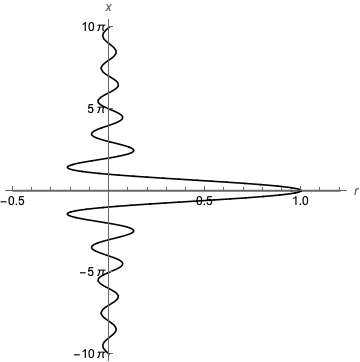
\includegraphics[scale=0.9]{img/PSet02-rxsinx-bifn.png}


\end{parts}

% \question (Backwards time) Consider a system $\dot{x} = f(x)$.  This is $\displaystyle\frac{dx}{dt} = f(x)$.  We have been reasoning about what happens to solutions $x(t)$ as $t\rightarrow \infty$.  This is sometimes referred to as the behavior of the variable $x$ in \emph{forward time}.  It is sometimes helpful to consider the behavior of $x$ in the past.  To think about where $x$ came from we can examine what would happen as time decreases towards $-\infty$.  %Thinking about \emph{backwards time}, we could redo all of our analyses for $t\rightarrow -\infty$. 

% One way this is often approached mathematically is to do a change of variables that reverses time in the system.  
% \begin{itemize}
% \itemsep0pt
% \item Create a new variable, $t_1 = -t$.  
% \item Rewrite the system in terms of $t_1$.  
% \item When $t\rightarrow -\infty$ we have $t_1 \rightarrow \infty$, so using our standard analysis methods we learn about the behavior of the system in backwards time.
% \end{itemize}
% \begin{parts}
% \item For the generic system above, $\displaystyle\frac{dx}{dt} = f(x)$, do the change of variables suggested and rewrite the system in terms of $t_1$ (show your steps).  Assume $x^*$ is a fixed point of $\displaystyle\frac{dx}{dt} = f(x)$.  Is it a fixed point of the new system (briefly justify your answer)?  If it is, identify its stability in the new system in terms of its stability in the original system.  
% \begin{solution}
% $\frac{dx}{dt} = f(x)$.  We want to find $\frac{dx}{dt_1}$ where $t_1 = -t$.  $\frac{dx}{dt_1} = \frac{dx}{dt}\frac{dt}{dt_1} = -\frac{dx}{dt}$.  So $\frac{dx}{dt} = - \frac{dx}{dt_1} = f(x)$.

% Our new differential equation is $\frac{dx}{dt_1} = -f(x)$.

% We assume $x^*$ is a fixed point of $\frac{dx}{dt} = f(x)$, so $f(x^*) = 0$.  That means $-f(x^*)$ is also zero, and $x^*$ is a fixed point of $\frac{dx}{dt_1} = -f(x)$ as well.

% In the new system, the sign of the vector field $\frac{dx}{dt_1}$ is exactly reversed from its sign in the old system.  That means that away from fixed points (where there is no flow) the direction of the flow is reversed.  The reversal in the direction of flow will lead to a reversal in the stability of all fixed points (stable fixed points become unstable, and unstable fixed points become stable).  For half-stable fixed points, a reversal in stability still results in a half-stable fixed point.  In that case, the stable and unstable sides of the fixed points will be exchanged.
% \end{solution}

% \item For the system $\displaystyle\frac{dx}{dt} = x(1-x)$, create a phase portrait for the forward time system.  Also create a phase portrait for the backward time system.
% \end{parts}



\question (Nondimensionalization practice) 
{\color{blue}\href{https://hollis.harvard.edu/primo-explore/fulldisplay?docid=01HVD_ALMA512272214860003941&context=L&vid=HVD2&lang=en_US&search_scope=everything&adaptor=Local%20Search%20Engine&tab=everything&query=any,contains,strogatz%20nonlinear&offset=0}{link to book on Hollis}}
%\begin{parts}
%\item 
Do 3.5.8.
%\item Do 3.6.5b.  Skip all of the other parts of this problem (you're using the equation from part a but don't need to do part a).  There is only one variable in this equation (time isn't involved).  Treat $m, g, \sin\theta, k, L_0, a$ as constants.  Let $u = x/x_0$ and proceed through the nondimensionalization process from there.
%\end{parts}

\question Consider the system $\dot x = r x - ax^2 - x^3$ where $a\in \mathbb{R}$.  When $a = 0$ we have the normal form for a supercritical pitchfork bifurcation.  Study the effects of the parameter $a$.
\begin{parts}
\item For each value of $a$ you can create a bifurcation diagram in the $rx$-plane.  As $a$ varies, these diagrams may be qualitatively different.  Provide a sketch or Mathematica/Python plot of each qualitatively different diagram.  \emph{Show your work / reasoning or make a note that the work was done computationally and can be found at the end of the pdf.}
\item To summarize your results, create an $ra$-plane (so each axis is a parameter).  Mark regions of the plane that have qualitatively different phase portraits.  Bifurcations are at the boundaries of the regions.  
\begin{itemize}
    \item Identify the types of bifurcations that occur. 
    \item Include a description of how you constructed this plot.
    \item Show work by hand to find an analytical expression for each bifurcation curve.

\end{itemize}
 
  

\emph{We are referring to this type of parameter-space plot as a \textbf{stability diagram}}.
\end{parts}


\question (3.7.5)  See the text for this question.  
\begin{parts}
\item Do this as written.  Find the dimensionless groups equal to $s$ and to $r$.
\item Do this as written, determining $r_c$.
\item Consider the three bifurcation diagrams below.

\hspace{-0.6in}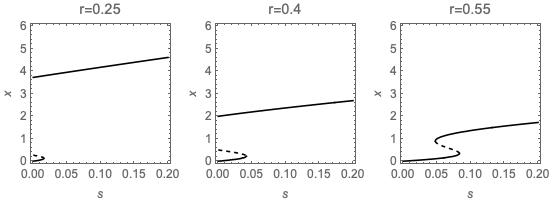
\includegraphics[width=\textwidth]{img/PSet02-375switch-bifn.png}

For each of these values of $r$, answer the question in the text.

\item Do this as written.

\item Do this as written.

\item The bifurcation diagrams in (c) correspond to straight lines on your plot in (e) at $r = 0.25$, $r=0.4$, and $r=0.55$.  What information from the bifurcation diagram appears in your stability diagram?  What information is lost?

\item The title of the problem was ``A biochemical switch'', where the switch refers to a single pulse of some signaling substance turning on a gene.  The gene then stays on even when the substance has disappeared.  According to your analysis, for what range of $r$ does the system have this kind of switch?  How can you see this from the stability diagram in (e)?

\end{parts}



%\question (4.5.3)  See the text for this question.


% \question (4.4.4) See the text for this question.  Show your work for each part. 

% Some context: see section 4.4 for a diagram of the setup.  We are applying a constant torque to the pendulum (a rotational version of force) and that torque is being balanced by gravity pulling the pendulum.  Once we add the spring, we have the spring helping gravity.  

% Usually a pendulum equation involves angular position, angular velocity, and angular acceleration (where angular acceleration is $\ddot{\theta}$).  We don't know how to deal with second derivatives (angular acceleration) at the moment, so we can only think about a case where $\dot{\theta}$ (the friction/damping/resistance to turning at the joint of the pendulum) is very large relative to $\ddot{\theta}$.  This is called the \emph{overdamped} limit.

% \emph{When analysing the system, assume $\theta$ is linearly increasing (so that the opposing torque at $4*\pi >$ opposing torque at $2\pi$).  The spring will be very stretched by the angle wrapping around, so $0$ and $2\pi$ are not equivalent here.  In this problem we have an angular variable and because of the spring, the physics is not equivalent at angles of $0$ and $2\pi$, so the actual angle (and not just the angle mod $2\pi$) matters.}


\end{questions}



\end{document}
